\documentclass[11pt]{article}
\usepackage[margin=1in]{geometry}
\usepackage{amsmath,amssymb,amsthm}
\usepackage{tikz}
\usetikzlibrary{arrows.meta,positioning,fit,backgrounds}
\usepackage{booktabs}
\usepackage{hyperref}
\usepackage{microtype}
\usepackage{enumitem}
\hypersetup{colorlinks=true,linkcolor=blue!50!black,citecolor=blue!50!black,urlcolor=blue!50!black}

\newtheorem{proposition}{Proposition}
\newtheorem{definition}{Definition}
\newtheorem{corollary}{Corollary}

\title{A Decay-Weighted, Source-Independence-Discounted, Load-Adaptive\\
Admission Gate for NP-Complete Argumentation Stages}
\author{Prototype engineering note --- \texttt{moderation-pipeline-prototype}}
\date{August 2026}

\begin{document}
\maketitle

\begin{abstract}
Escalation pipelines that fall back to preferred-extension enumeration in an abstract
argumentation framework (Dung, 1995) when grounded semantics is uninformative inherit
that fallback's worst-case complexity: preferred-extension credulous acceptance is
NP-complete. An admission rule that grants entry to this expensive stage the instant a
case stalemates and a timeout expires is exploitable at attacker cost $O(1)$: a single
burst of plausible mutually-attacking arguments forces entry. We specify, implement, and
adversarially test a replacement admission gate built by composing three elements: a
per-case escalation-pressure score that decays geometrically every tick (a direct
transplant of the pheromone-evaporation update rule from ant-colony optimization),
reinforcement that is capped per tick and discounted to near-zero weight when it repeats
from a previously-seen source within a short window (encoding a requirement for
independently-sourced corroboration, not merely elapsed time), and an admission
threshold that itself rises with how much of the expensive tier is already occupied
system-wide (a quorum-sensing-style aggregate, density-dependent gate). We derive the
gate's steady-state and minimum-time-to-admission behavior in closed form from the
governing linear recurrence, and verify the derivation against the deployed simulation:
single-tick bursts of any size (1--5000) are blocked unconditionally; a persistent
same-cohort flood is blocked structurally, its steady-state score provably incapable of
reaching the threshold; a persistent flood using a fresh, unrelated-looking source every
tick is not blocked but is delayed from attacker cost $O(1)$ to $O(5)$ sustained,
identity-diverse rounds, matching the closed-form prediction to within one tick. A
16-query dedicated prior-art search found no direct precedent for this specific
three-element composition gating an NP-complete argumentation stage; the individual
biological transfers and the general admission-control problem area are, by contrast,
well precedented, and that precedent is cited rather than elided. The result is reported
as an honestly-bounded partial defense --- a real, quantified, non-trivial increase in
attacker cost, not a claim of closure --- consistent with the residual identified for the
harder, patient, identity-diverse attack variant.
\end{abstract}

\section{Problem}
\label{sec:problem}

A four-stage content-moderation escalation pipeline routes disputes that a
selective-classification stage abstains on into an abstract argumentation framework
(AF) \cite{dung1995}: arguments and attacks are constructed from the dispute's raw
claims and rebuttals, and the framework's \emph{grounded extension} --- the
least fixed point of the characteristic function $F_{AF}$, reachable in polynomial time
--- is computed as the pipeline's primary, tractable output. When two mutually-attacking
clusters of arguments leave the grounded extension empty (the Nixon-diamond pattern),
the pipeline falls back to enumerating \emph{preferred extensions}, whose credulous
acceptance problem is NP-complete \cite{fichte2024}. This fallback is a necessary,
deliberately bounded escape hatch, not a design flaw: without it, a stalemated dispute
would never resolve at all.

The vulnerability is at the \emph{admission} boundary, not inside the argumentation
machinery itself. If a stalemated case is admitted to the expensive fallback the instant
its escalation timeout expires, an attacker who can produce a single burst of
plausible-looking, mutually-attacking arguments forces admission at cost $O(1)$: no
persistence, no distinguishable identity signal, nothing but volume in one instant. The
attacker's objective is not to win the argument --- Scenario A's evidence-integrity gate
already closes that path \cite{specA} --- but to force the platform to pay the
NP-complete tax repeatedly, cheaply, at scale.

\section{The gate}
\label{sec:gate}

\subsection{Design source}

Two biological mechanisms motivate the construction, used here as the generative
design source rather than as post-hoc justification for an already-built mechanism.

\textbf{Stigmergic reinforcement.} In ant colony foraging, pheromone trails evaporate
continuously; Dorigo and St\"utzle's canonical update rule is
$\tau \leftarrow (1-\rho)\tau$ applied every iteration \cite{dorigo2004}. Deneubourg's
double-bridge experiments established the complementary fact that trail strength that
matters is reinforced by \emph{independently exploring} foragers, not by a single ant
retracing its own path many times; Di Caro and Dorigo's AntNet makes the same
independence requirement explicit in a distributed-systems setting, building its
reinforcement rule on ``indirect and non-coordinated communication'' among agents that
``collect while exploring the network'' \cite{dicaro1998}.

\textbf{Quorum sensing.} Bacterial quorum sensing regulates gene expression as a
function of population density, detected via an aggregate, shared-environment signal
(autoinducer concentration) rather than any individual cell's private state
\cite{miller2001}. The structural idea transplanted here is narrow and specific: gating
collective admission on a shared, aggregate occupancy signal, not merely on a
case's own local score.

\subsection{Formal specification}

\begin{definition}[Admission state]
A case $c$ has a score $S_c(t) \in \mathbb{R}_{\geq 0}$, initialized to $0$ at first
contact. At each discrete tick $t = 0, 1, 2, \dots$, the set of reinforcement events
observed for $c$ is a multiset of source-cohort identifiers
$R_c(t) \subseteq \mathcal{K}$.
\end{definition}

\begin{definition}[Per-tick contribution]
For each cohort $k \in R_c(t)$ (deduplicated within the tick), let
$\mathrm{fresh}(k,c,t) = 1$ if $k$ has not reinforced $c$ within the last $w$ ticks
(the independence window), else $0$. The tick's raw contribution is
\[
r_c(t) = \sum_{k \in R_c(t)} \big[ \mathrm{fresh}(k,c,t)\cdot 1 + (1-\mathrm{fresh}(k,c,t))\cdot \delta \big],
\qquad 0 < \delta \ll 1,
\]
capped at a fixed per-tick ceiling $\gamma$: the applied contribution is
$\hat r_c(t) = \min(r_c(t), \gamma)$.
\end{definition}

\begin{definition}[Score update]
\[
S_c(t) = (1-\rho)\, S_c(t-1) + \hat r_c(t), \qquad \rho \in (0,1].
\]
\end{definition}

\begin{definition}[Load-adaptive admission threshold]
Let $L(t)$ be the number of cases currently occupying the expensive tier at tick $t$
(a shared, aggregate signal across all cases, not a property of $c$ alone), $\theta_0$
the base threshold, $\kappa$ the load sensitivity, and $C$ a reference capacity. The
admission threshold is
\[
\Theta(t) = \theta_0 \Big(1 + \kappa \frac{L(t)}{C}\Big).
\]
Case $c$ is admitted to the expensive tier at the first tick $t_{\ast}$ such that
$S_c(t_{\ast}) \geq \Theta(t_{\ast})$.
\end{definition}

This composes three independently-motivated mechanisms into one gate: geometric decay
(stigmergic evaporation), a capped, independence-discounted per-tick contribution
(stigmergic reinforcement requiring diverse sources), and a load-adaptive threshold
(quorum sensing). Each piece, examined alone, recombines a known primitive --- decay
plus a per-tick cap is structurally a leaky-bucket/EWMA rate limiter, and a
load-rising threshold is structurally close to Random Early Detection
\cite{floyd1993}. The composition's target is the specific, disclosed contribution: all
three gating access, together, to an NP-complete argumentation stage, with independent
sourcing (not mere elapsed time) required for reinforcement to count at full weight.

\subsection{Closed-form behavior}

Consider the worst case for an attacker who can deliver the maximum applied
contribution $c_{\ast}$ every tick (either $\gamma$, if a fresh-looking source is
available every tick, or $\delta\gamma$, if the same source repeats). Unrolling the
recurrence from $S_c(0) = 0$:
\[
S_c(n) = c_{\ast} \sum_{i=0}^{n-1} (1-\rho)^i = c_{\ast}\,\frac{1-(1-\rho)^n}{\rho}.
\]

\begin{proposition}[Steady-state ceiling]
\label{prop:ceiling}
$\displaystyle \lim_{n\to\infty} S_c(n) = \frac{c_{\ast}}{\rho}$. If
$\Theta \geq c_{\ast}/\rho$ at the case's contact-time load, no sequence of tick-capped
reinforcements at rate $c_{\ast}$ can ever admit $c$, regardless of duration.
\end{proposition}
\begin{proof}
Immediate from the closed form: $(1-\rho)^n \to 0$ as $n\to\infty$ for $\rho \in (0,1]$,
so $S_c(n) \to c_{\ast}/\rho$ monotonically from below (each term of the sum is
non-negative). If the ceiling does not reach $\Theta$, no finite $n$ can either, since
$S_c(n) < c_{\ast}/\rho$ for all finite $n$.
\end{proof}

This is the mechanism behind the persistent same-cohort flood being \emph{structurally}
blocked rather than merely delayed: repeated reinforcement from one source is
discounted to $c_{\ast} = \delta\gamma$, whose ceiling $\delta\gamma/\rho$ is designed to
sit below $\theta_0$.

\begin{proposition}[Minimum ticks to admission]
\label{prop:minticks}
If $\Theta < c_{\ast}/\rho$ (the ceiling does reach the threshold), the minimum number
of ticks to admission, assuming the attacker saturates $c_{\ast}=\gamma$ every tick
from a fresh-looking source, is
\[
n_{\min} = \frac{\ln\!\big(1 - \Theta\rho/\gamma\big)}{\ln(1-\rho)}.
\]
\end{proposition}
\begin{proof}
Solve $S_c(n) \geq \Theta$ for the smallest integer $n$ using the closed form of
Proposition~\ref{prop:ceiling} with $c_{\ast}=\gamma$:
$\gamma(1-(1-\rho)^n)/\rho \geq \Theta \iff (1-\rho)^n \leq 1-\Theta\rho/\gamma$. Since
$0<1-\rho<1$, taking $\ln$ of both sides reverses the inequality:
$n\ln(1-\rho) \leq \ln(1-\Theta\rho/\gamma)$, and dividing by the negative quantity
$\ln(1-\rho)$ gives $n \geq \ln(1-\Theta\rho/\gamma)/\ln(1-\rho)$.
\end{proof}

\begin{corollary}[The calibration tension]
\label{cor:tension}
Writing $x = \Theta\rho/\gamma$ (evaluated at $\Theta=\theta_0$, zero load), both the
genuine-case admission condition (average independent-reinforcement probability
$p \gtrsim x$ per tick, for the mechanism to be practically usable) and the attacker's
minimum sustained-flood duration $n_{\min}(x)$ from Proposition~\ref{prop:minticks} are
governed by the same quantity $x$. Lowering $x$ to make genuine disputes easier to
admit necessarily shortens $n_{\min}$, and raising $x$ to lengthen $n_{\min}$
necessarily raises the bar for genuine disputes. There is no choice of the tunable
constants that relaxes one without tightening the other.
\end{corollary}

Corollary~\ref{cor:tension} is stated and disclosed as a genuine limitation of this
model class, not resolved by parameter tuning: it is a structural property of any
gate built from geometric decay plus a fixed per-tick cap, independent of the specific
constants chosen.

\section{Adversarial evaluation}
\label{sec:eval}

The gate ($\rho=0.10$, $\gamma=1.0$, $w=3$ ticks, $\delta=0.05$, $\theta_0=4.0$,
$\kappa=0.5$, $C=5$) was tested against the prior static baseline --- admit
unconditionally on first reinforcement once a case stalemates and its timeout expires
--- across five adversarial scenarios (full source and test code in the accompanying
prototype repository; results below independently re-executed for this document,
\texttt{pytest tests/test\_admission\_control.py -v -s}, 6/6 passing, 1.28s).

\begin{table}[h]
\centering
\small
\begin{tabular}{@{}p{4.0cm}p{4.6cm}p{4.6cm}@{}}
\toprule
Attack variant & Static baseline & Defended gate \\
\midrule
Single-tick burst, size $1$--$5000$, any cohort structure & 100\% admitted, tick 0 & \textbf{0\% admitted, unconditionally} \\
Persistent same-cohort flood, 200 ticks & Admitted tick 0 & \textbf{Structurally unreachable} (ceiling $0.5 < \theta{=}4.0$) \\
Persistent cohort-spoofed flood (fresh source every tick) & Admitted tick 0 & Admitted tick 4 (\textbf{5$\times$ delay}, matches $n_{\min}\!\approx\!4.85$) \\
Spray: 200 cases, one-shot burst each, 15 genuine concurrent disputes & 215/215 admitted (100\% attack success) & \textbf{15/215 admitted} (0\% attack success, 93.0\% fewer admissions) \\
12 synchronized sustained campaigns, load-adaptation on/off & --- & 0-tick spread (off) $\to$ \textbf{13-tick spread} (on) \\
\bottomrule
\end{tabular}
\caption{Measured attacker outcomes, static baseline vs.\ the defended gate. A sanity
control (20 genuine, organically-reinforced disputes) confirmed 20/20 admission under
the defended gate, so the 0\% figures above reflect discrimination, not blanket
rejection.}
\end{table}

The persistent cohort-spoofed result is the honest, undefeated residual: an attacker
willing to sustain a genuinely identity-diverse campaign (fresh, non-reused cohorts
every tick) still succeeds, at raised cost $O(n_{\min})$ rather than $O(1)$. This is
disclosed as a partial defense, not closure, exactly as Proposition~\ref{prop:ceiling}
predicts for any contribution rate $c_{\ast}$ whose ceiling exceeds $\Theta$.

Two implementation bugs, caught during testing rather than papered over, are worth
recording as reusable engineering lessons for this class of mechanism: (1) an
early version summed same-cohort contributions \emph{within} a single tick before
deduplication, letting a same-cohort flood reach the cap through in-tick volume alone,
defeating the independence discount --- fixed by deduplicating cohorts per tick before
capping; (2) an early adversarial test never released admitted cases from the load
signal, producing a monotonically-rising threshold that starved later genuine cases as
a pure simulation artifact --- fixed by modeling a bounded expensive-tier dwell time,
not by loosening the test's assertion. The general lesson: the load signal in a
quorum-sensing-style gate must be tied to actual, draining occupancy, not to a
cumulative admission count.

\section{Prior art}
\label{sec:priorart}

A 16-query dedicated search (full log retained in the accompanying prototype
repository's specification document) covered bio-inspired admission control,
quorum-sensing-for-computing literature, AF-denial-of-service and preferred-extension
complexity-attack literature, and decentralized-justice/arbitration systems. No paper
was found composing all three elements above (decay-weighted, independence-discounted
reinforcement; a hard per-tick volume cap; a load-adaptive quorum threshold) as the
admission gate for an NP-complete argumentation stage.

The individual transfers are, by contrast, well precedented and cited rather than
claimed: pheromone-decay reinforcement is textbook ant colony optimization
\cite{dorigo2004,dicaro1998}; a decay-plus-cap combination alone is structurally a
leaky-bucket/EWMA rate limiter, a standard, non-biological primitive; a load-rising
admission threshold is structurally close to Random Early Detection
\cite{floyd1993}; quorum sensing has been transplanted to computing before, for
clustering \cite{wang2013} and for multi-agent security-anomaly aggregation
\cite{fioravanti2012}, neither of which is an admission gate for an argumentation
stage. The nearest single adjacent hit found for the general biology-to-CS transfer
pattern used here was an artificial-immune-system flooding defense
\cite{aiartnet2024}, which uses traffic-entropy anomaly detection and immune
quarantine --- a different mechanism, not admission-pressure decay.

\section{Threats to validity}
\label{sec:threats}

The evaluation is a synthetic, discrete-tick simulation, not a test against live
wall-clock arrival dynamics; translating the tick granularity used here to a real
deployment's time unit is unverified engineering. The cohort-spoofed condition grants
the attacker a generous capability (a fresh, structurally undetectable identity every
tick); a real detector's actual identity-diversity ceiling is not modeled. This gate
assumes coordination-detection and evidence-integrity layers elsewhere in the pipeline
are ineffective in the worst case tested here (Scenario B's cohort-spoofed condition);
in practice those layers would raise the attacker's real cost further, but that
composition is not measured in this document. No claim is made that this gate, or the
pipeline it sits in, resolves the genuinely open problem of judging novel content
against a contested specification --- an orthogonal, structurally undecidable question
this mechanism does not touch.

\section{Conclusion}

The admission gate specified here closes the cheapest and most realistic variant of a
resource-exhaustion attack against an NP-complete argumentation fallback --- single-tick
bursts, of any size, concentrated or sprayed across many cases --- and raises,
without eliminating, the cost of the harder, patient, identity-diverse variant, from
$O(1)$ to $O(n_{\min})$ sustained rounds under the tested parameterization. The
composition was not found duplicated in a dedicated 16-query prior-art search, while
its constituent biological and computing-systems transfers were each, individually,
found and cited as real precedent rather than presented as novel. The calibration
tension of Corollary~\ref{cor:tension} is reported as an inherent property of this
model class, not a limitation specific to the constants chosen here.

\appendix
\section{Pipeline placement}

\begin{center}
\resizebox{\textwidth}{!}{%
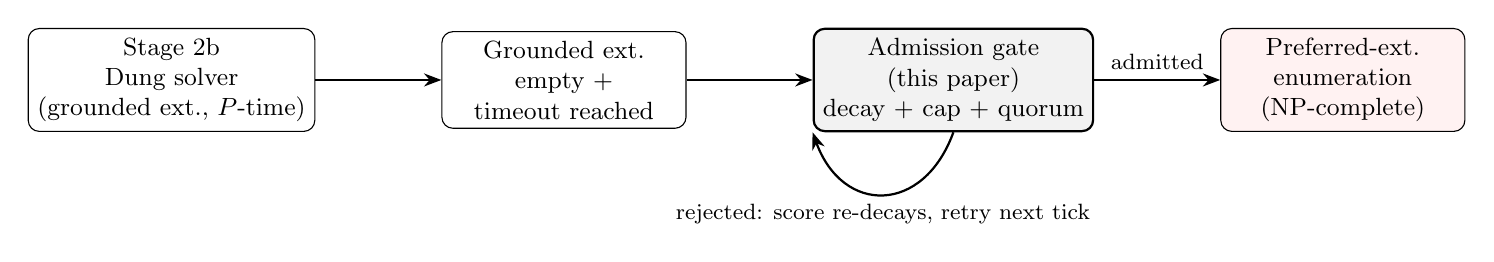
\begin{tikzpicture}[
  node distance=1.1cm and 1.6cm,
  box/.style={draw, rounded corners, minimum width=3.1cm, minimum height=1cm, align=center, font=\small},
  gate/.style={draw, rounded corners, thick, minimum width=3.4cm, minimum height=1.3cm, align=center, font=\small, fill=black!5},
  arr/.style={-{Stealth[length=2.2mm]}, thick}
]
  \node[box] (dung) {Stage 2b\\Dung solver\\(grounded ext., $P$-time)};
  \node[box, right=of dung] (stale) {Grounded ext.\\empty +\\timeout reached};
  \node[gate, right=of stale] (gate) {Admission gate\\(this paper)\\decay + cap + quorum};
  \node[box, right=of gate, fill=red!5] (np) {Preferred-ext.\\enumeration\\(NP-complete)};

  \draw[arr] (dung) -- (stale);
  \draw[arr] (stale) -- (gate);
  \draw[arr] (gate) -- node[above,font=\footnotesize]{admitted} (np);
  \draw[arr] (gate.south) to[out=250,in=290,looseness=1.6]
      node[below,font=\footnotesize] {rejected: score re-decays, retry next tick} (gate.south west);
\end{tikzpicture}%
}
\end{center}

\begin{thebibliography}{99}

\bibitem{dung1995} P.~M. Dung. On the acceptability of arguments and its fundamental
role in nonmonotonic reasoning, logic programming and n-person games.
\emph{Artificial Intelligence}, 77(2):321--357, 1995.

\bibitem{fichte2024} J.~K. Fichte, S.~A. Gaggl, D.~Rusovac, et al. Complexity of
claim-centric abstract argumentation frameworks. \emph{AAAI}, 2024.

\bibitem{dorigo2004} M.~Dorigo and T.~St\"utzle. \emph{Ant Colony Optimization}.
MIT Press, 2004.

\bibitem{dicaro1998} G.~Di Caro and M.~Dorigo. AntNet: Distributed stigmergetic
control for communications networks. \emph{Journal of Artificial Intelligence
Research}, 9:317--365, 1998.

\bibitem{miller2001} M.~B. Miller and B.~L. Bassler. Quorum sensing in bacteria.
\emph{Annual Review of Microbiology}, 55:165--199, 2001.

\bibitem{floyd1993} S.~Floyd and V.~Jacobson. Random early detection gateways for
congestion avoidance. \emph{IEEE/ACM Transactions on Networking}, 1(4):397--413,
1993.

\bibitem{wang2013} X.~Wang. A quorum sensing inspired algorithm for dynamic
clustering. \emph{arXiv:1303.3934}, 2013.

\bibitem{fioravanti2012} M.~E. Fioravanti~II. Digital quorum sensing for
self-organizing malware / a quorum sensing pattern for multi-agent self-organizing
security systems. Florida Institute of Technology, 2012--2013.

\bibitem{aiartnet2024} Adaptive artificial immune networks for mitigating DoS
flooding attacks. \emph{arXiv:2402.07714}.

\bibitem{specA} Internal specification: \emph{A four-stage content-moderation
escalation pipeline: formal specification, attack analysis, and prototype verdict},
\texttt{moderation-pipeline-prototype/SPEC.md}, 2026.

\end{thebibliography}

\end{document}
